

\documentclass[DIV=calc, paper=a4, fontsize=11pt]{scrartcl}
\usepackage{makeidx}
\usepackage{graphicx}
\usepackage{flushend}
\usepackage{amssymb}


\usepackage{lmodern}
\usepackage[left=1.5cm,right=1.5cm,top=2.5cm,bottom=2cm]{geometry}
\usepackage{float}		
\bibliographystyle{plain} 
\pagestyle{plain} 
\pagenumbering{arabic}
\usepackage{fancyhdr} 	
\usepackage[T1]{fontenc}
\usepackage[utf8]{inputenc}
\usepackage[spanish]{babel}
\usepackage[spanish,es-tabla]{babel}
\usepackage{hyperref}
\usepackage{graphicx}
\usepackage{siunitx}
\usepackage{lipsum}
\usepackage[protrusion=true,expansion=true]{microtype}
\usepackage{amsmath,amsfonts,amsthm}
\usepackage[svgnames]{xcolor}
\usepackage[svgnames]{xcolor}
\usepackage{booktabs}
\usepackage{fix-cm}
\usepackage{multicol}
\usepackage{url}
\usepackage{cancel}
\usepackage{subfig}
\bibliographystyle{unsrt}

\newenvironment{Figura}
  {\par\medskip\noindent\minipage{\linewidth}}
  {\endminipage\par\medskip}

\usepackage{sectsty}
\allsectionsfont{\usefont{OT1}{phv}{b}{n}}
\usepackage{fancyhdr}
\spanishdecimal{.}
\pagestyle{fancy}
\usepackage{lastpage}
\lhead{}
\chead{}
\rhead{}
\lfoot{}
\cfoot{}
\rfoot{\footnotesize Page \thepage\ of \pageref{LastPage}}
\renewcommand{\headrulewidth}{0.0pt}
\renewcommand{\footrulewidth}{0.4pt}
\usepackage{lettrine}
\newcommand{\initial}[1]{\lettrine[lines=3,lhang=0.3,nindent=0em]{
\color{DarkGoldenrod}{\textsf{#1}}}{}}
\usepackage{titling}
\newcommand{\HorRule}{\color{DarkGoldenrod} \rule{\linewidth}{1pt}}
\pretitle{\vspace{-120pt} \begin{flushleft} \HorRule \fontsize{22}{35} \usefont{OT1}{phv}{b}{n} \color{DarkRed} \selectfont}
\title{Práctica 2. \\ %Aquí va el nombre de la práctica 
Radiometría} %Numero de la práctica 
\posttitle{\par
\end{flushleft}
\vskip 0.5em}
\preauthor{\begin{flushleft}\large \lineskip 0.5em \usefont{OT1}{phv}{b}{sl} \color{DarkRed}}
\author{Angel Yair García Pérez \\
Misael Iván Macías Márquez\\
Teodora Irene Ortíz Cruz\\
\small{teodora625@ciencias.unam.mx}\\}
\postauthor{\footnotesize \usefont{OT1}{phv}{m}{sl} \color{Black}
\vspace*{0.1cm} 
Facultad de Ciencias, UNAM
\par\end{flushleft}\HorRule}
\date{04 de Abril del 2022\\Semestre 2022-2}
\begin{document}
\maketitle
\definecolor{carmine}{rgb}{0.59, 0.0, 0.09}
\begin{abstract}

  \textcolor{carmine}{Resumen:} Se determinó el comportamiento para fuentes de luz LED plana, LED y lasér. Para ello se midió el voltaje de la luz incidente con un radiómetro y la distancia entre la fuente de luz incidente y el fotoreceptor con la regla que incluía el riel óptico. Se hizo un análisis gráfico con el cual se llegó a que una fuente LED plana aproxima la Ley coseno de Lambert, también se obtuvo que el LED se puede aproximar como fuente puntual y para puntos cercanos se puede considerar al láser como una fuente de luz colimada, ya que se obtuvo la siguiente ecuación $\ln{V}=(-0.07\pm0.01)\ln{R}+3.82$, la distancia de los puntos cercanos depende de que tan buena se quiera la aproximación.
\end{abstract}
\section*{\textcolor{carmine}{Introducción.}}
El propósito de este experimento es estudiar y determinar el comportamiento de propagación de la luz de ciertas fuentes comunes y comparar los resultados que se obtengan con las debidas incertidumbres \cite{ManualP1}. Debido a lo anterior, la importancia de este trabajo se centra en resaltar las diferencias entre algunas fuentes de luz. Para ello se pondrán aprueba la ley del coseno de Lambert y la ley de inverso cuadrado\cite{Manual}.\\Con base a los estudios realizados en 2009 por Luis Diego Marín Naranjo \cite{Reporte} se espera que  el LED se comporte como una fuente de luz puntual mientras que el lasér se comporte como una fuente de luz colimada en distancias pequeñas. Por otro lado a partir de la misma literatura se tiene la hipótesis de que la fuente de luz LED plana cumple con la ley de coseno de Lambert  


\subsection*{\textcolor{carmine}{Fotodiodo.}}%El fotodiodo va antes
Un fotodiodo es un dispositivo semiconductor que convierte luz en una corriente eléctrica mediante el efecto fotoeléctrico. Cuando se polariza inversamente, la corriente puede ser medida como un voltaje a través de una resistencia.
Bajo ciertas condiciones de operación, la corriente generada por el fotodiodo $C_f$ (número de electrones que fluyen por el circuito) será linealmente proporcional al número de fotones que incide en la unión $\phi_fA_f$, y como la irradiancia $I_f$ es la densidad de flujo de radiación por unidad de área, también será proporcional a la irradiancia que recibe\cite{Manual}.
\begin{equation*}
    C_f = k \frac{\phi_f}{A_f}= kI_f
\end{equation*}
La forma más común de medir la irradiancia en un fotodiodo es a través del voltaje $V$ producido por su corriente de salida ($C_f$) por medio de una resistencia $R$, la cual por la Ley de Ohm esta dada por \cite{Manual}:
\begin{equation}
    V= C_f R = k R I_f
\end{equation}
\subsection*{\textcolor{carmine}{Ley coseno de Lambert.}}

Un radiador Lambertiano es aquella superficie real o imaginaria cuya intensidad radiante es independiente de la dirección y que también obedece la ley coseno de Lambert.\\
Esta ley dice que la irradiancia $I$ proveniente de un área y emitida sobre una superficie $A$ varía con el coseno del ángulo $\theta$ entre la dirección de propagación y la normal de la superficie como se puede ver en la Figura 1, también se puede escribir como \cite{book}:
\begin{equation*}
    I = I_0 \cos{\theta}
\end{equation*}
\begin{equation*}
    \frac{I}{I_0} = \cos{\theta}
\end{equation*}

y sustituyendo la ecuación 1:

\begin{equation}
    \therefore \hspace{0.3cm}  \cancel{\frac{kR}{kR}}\frac{V}{V_0} =V_n= \cos{\theta}
\end{equation}

linealizando la ecuación 2 se obtiene:

\begin{equation}
    \cos^{-1}{V_n} = \theta
\end{equation}

donde la ecuación 3 es de la forma $y=mx+b$ con $y=\cos^{-1}{V_n}$, $m=1$, $x=\theta$ y $b=0$.

\begin{figure}[h!]
    \centering
    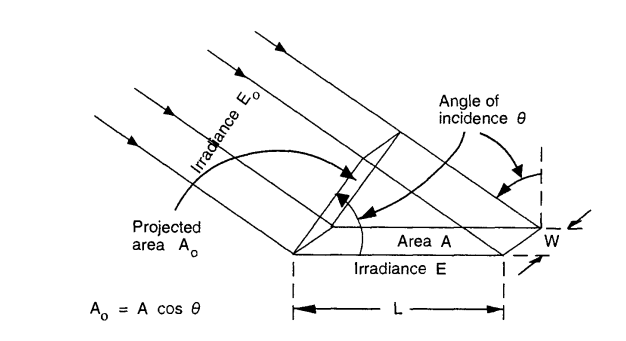
\includegraphics[scale=0.5]{diagrama lambert.PNG}
    \caption{\textbf{Diagrama de la ley de coseno de Lambert.} En ella se pueden observar el haz de luz colimada que incide en un área $A$ y con ello se puede obtener un área proyectada $A_{0}$ a la que se le asocia una irradiancia $I_{0}$ tal que $A_{0}=A\cos{\theta}$\cite{book}.}
\end{figure}

\subsection*{\textcolor{carmine}{Ley del inverso al cuadrado.}}
Si se considera un haz de luz que incide de forma perpendicular a la superficie se tiene que la irradiancia se define como $I= d^2\phi/d\omega ds$ y por definición de ángulo sólido ($d\omega = da_0/R^2$):
\begin{equation*}
    I_D = \frac{Id \omega}{da_0 } = \frac{I \cancel{da_0}}{\cancel{da_0} R^2} = \frac{I}{R^2}
\end{equation*}o bien asumiendo que la irradiancia $I$ es constante sobre la superficie de incidencia se tiene que:
\begin{equation}
    I_D = \frac{K}{R^2}
\end{equation}

con $K$ una constante\cite{book}.

Linealizando la ecuación 4 usando propiedades de los logaritmos se tiene:

\begin{equation}
    \ln{I_D}= -2\ln{R} + \ln{K} 
\end{equation}

donde la ecuación 5 es de la forma $y=mx+b$ con $y=\ln{I_D}$, $m=-2$, $x=\ln{R}$ y $b=\ln{K}$.


\section*{\textcolor{carmine}{Desarrollo Experimental.}}
\subsection*{\textcolor{carmine}{Parte I.}}
En la mesa del laboratorio se conectó un radiómetro y un LED plano que estaban sobre una mesa óptica, como se muestra en la Figura 2, alrededor del arreglo experimental se colocaron tablas oscuras para no permitir el paso de luz que entraba por la abertura de una de las ventanas  del laboratorio. Se midió el voltaje con el radiómetro sin que la fuente de Lambert estuviera encendida, dicho valor fue de $0.02V$ y es el ruido de las medidas. Con el arreglo experimental montado se comenzaron a medir los voltajes asociando una incertidumbre que iba de $0.05V$ hasta $0.01V$, se partió de un ángulo de $0^{\circ}$, los ángulos tienen una incertidumbre de apreciación de $2.5^{\circ}$, para poder mover el ángulo se utilizó una lampara de celular y se giro la fuente cada $5^{\circ}$ hasta llegar a $85^{\circ}$.\\
\begin{figure}[H]
    \centering
    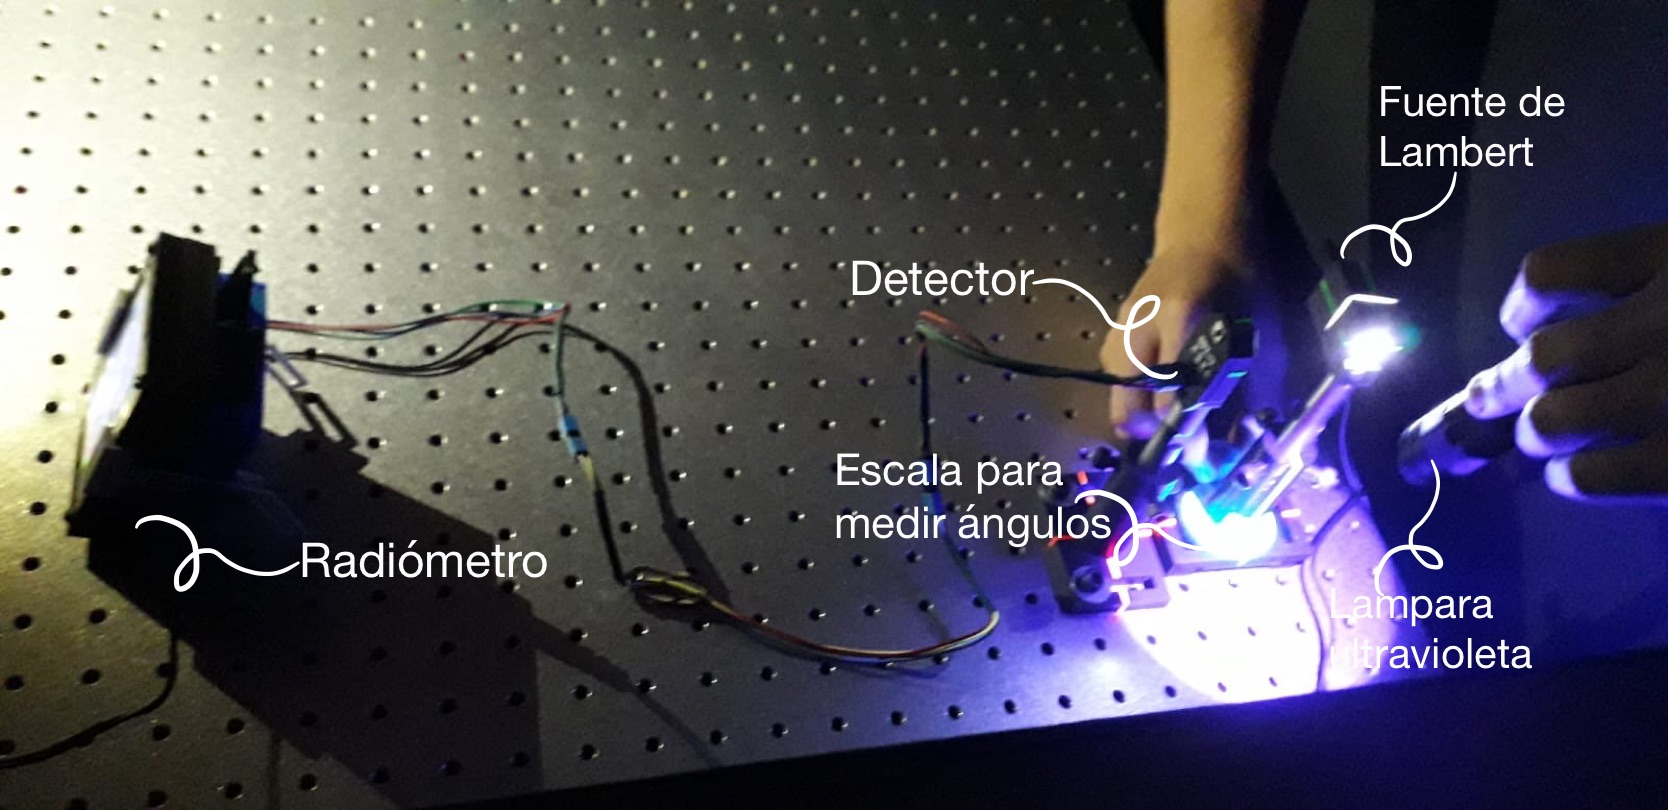
\includegraphics[width=8cm]{Imagen/7F90E32E-999D-435F-A061-F83648BB0EDF.jpeg}
    \caption{\textbf{Arreglo experimental 1.}En el se muestra al detector conectado al radiómetro frente a la fuente LED plana que emite luz, además se muestra como se utilizó la lampara de rayos UV.}
    \label{fig:my_label}
\end{figure}
\subsection*{\textcolor{carmine}{Parte II.}}
Se utilizó el riel óptico con escala y una fuente de luz como se muestra en la Figura 3(a), en este caso un LED, el experimento consistió en tomar medidas del voltaje mientras el detector se iba alejando. Se utilizó la lampara de luz UV para alumbrar la escala y medir la distancia a la que estaba el detector, la cual tenía una incertidumbre de apreciación de $\pm 0.05cm$. Con un vernier se midió que la fuente se encontraba $(1.8\pm0.05)cm$ recorrido con respecto al 0. Se colocaron las tablas oscuras para rodear el arreglo experimental y al igual que el primer experimento se tomo la medida del ruido con el radiómetro y la fuente de luz apagada, el valor medido fue de $0.02V$ siendo consistente con lo obtenido antes. 
Al conectar la fuente se esperó unos minutos a que se estabilizara, después se comenzaron a registrar las medidas de voltaje conforme el detector se alejaba, en la parte mas cercana a la fuente se tomaron más medidas. Se obtuvieron 20 datos.\\
Después se utilizó el riel óptico con escala y se colocó un láser como fuente de luz como se muestra en la Figura 3(b), el cual estaba a $(1.8cm\pm0.05cm)$ del $0$ de la escala del riel óptico, se siguió el mismo procedimiento que en la segunda parte excepto que en esta parte era necesario alinear el láser con el detector cada vez que se alejaba. Se tomaron 20 datos.
\begin{figure}[H]
 \centering
  \subfloat[\textbf{Arreglo experimental 2.} Se muestra el montaje el arreglo experimental para la segunda parte del experimento.]{
   \label{f:Arreglo 2}
    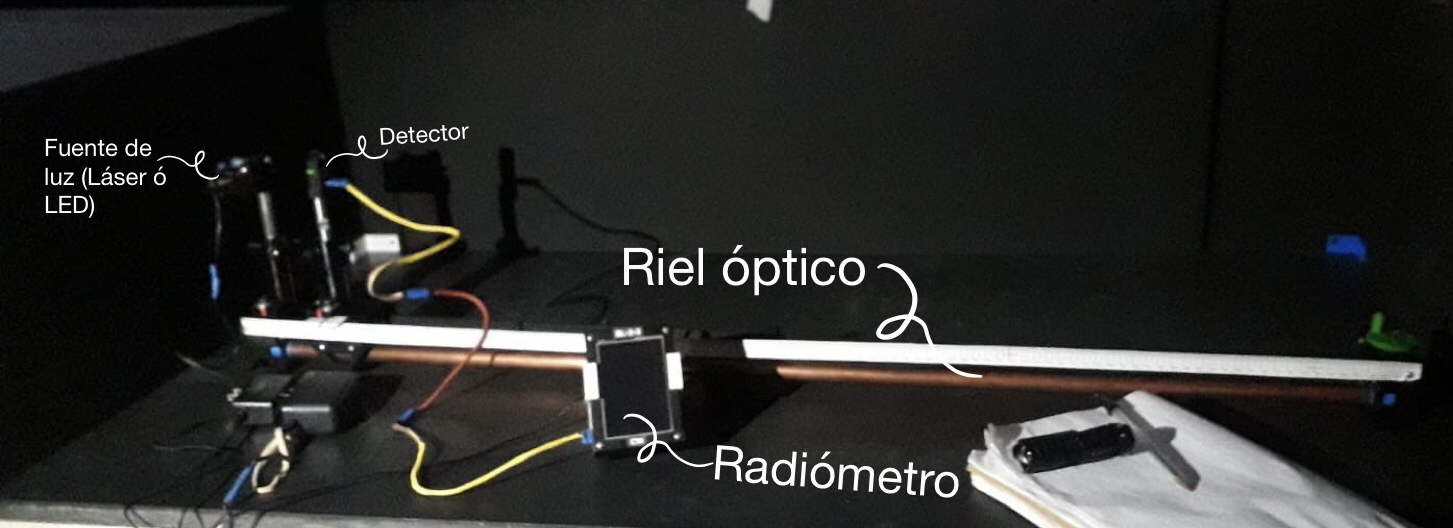
\includegraphics[width=0.5\textwidth]{Imagen/32C4A502-9E30-4F96-84E7-5965710E3055.jpeg}}
    \subfloat[\textbf{Láser-Detector.}]{
    \label{f:Lasér}
    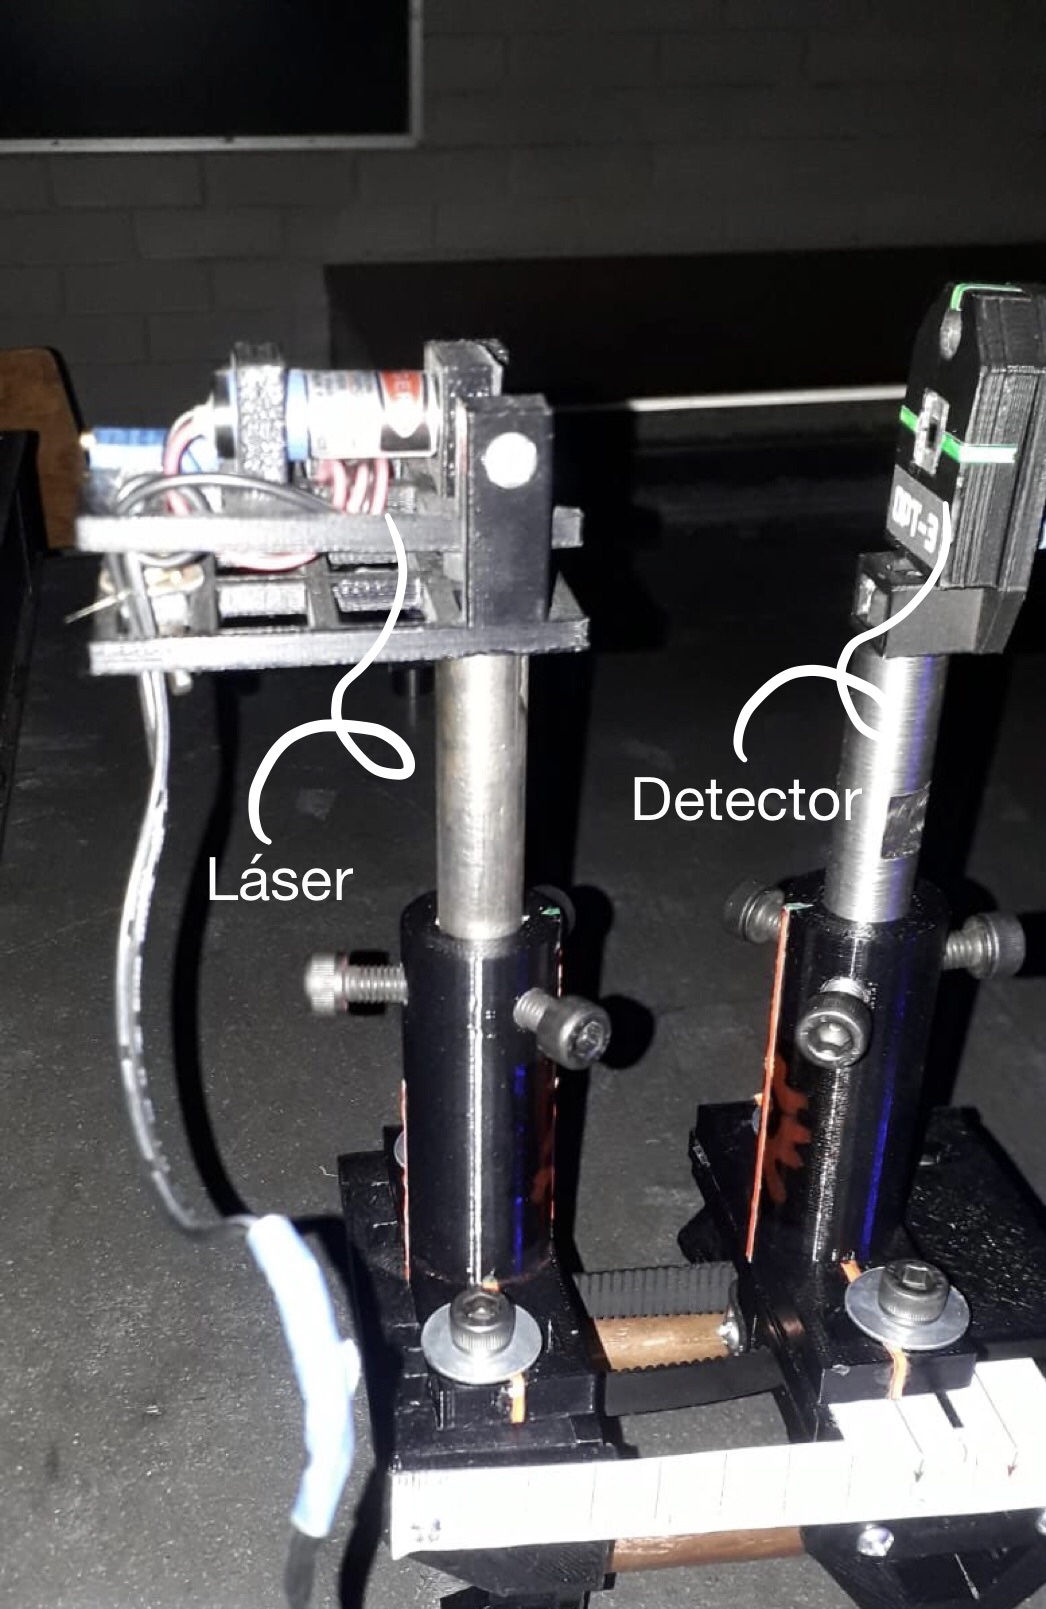
\includegraphics[width=0.11\textwidth]{Imagen/99FCF586-F033-4965-86D0-FFA9F6E2D038.jpeg}}
 \caption{Se muestra el arreglo experimental para la segunda parte, donde se puede ver el radiómetro conectado al detector frente a la fuente y el la figura 3(b) se puede ver con más detalle cuando se utilizo como fuente el láser.}
 \label{f:Segunda Parte}
\end{figure}
\section*{\textcolor{carmine}{Resultados y Discusión.}}

\subsection*{\textcolor{carmine}{PARTE I.}}

Tanto la distancia $L$ como el voltaje $V$ se encuentran desplazados por una constante con incertidumbre por lo que se tiene que propagar que es básicamente duplicar la incertidumbre de medición ya que se midieron con los mismos instrumentos.


Para los voltajes normalizados $V_n$ la incertidumbre se propagó fácilmente dividiendo la incertidumbre del voltaje por la misma constante que se utilizó para normalizar.


Utilizando la ecuación 3, $y= \cos^{-1}{V_n}$, entonces por la ley de derivación para propagación de incertidumbres:

\begin{equation*}
    \delta y = \sqrt{\left(\frac{\partial y}{\partial V_n} \delta V_n\right)^2} =\left| \frac{\partial y}{\partial V_n}\right| \delta V_n = \frac{\delta V_n}{\sqrt{1-V_{n}^{2}}} 
\end{equation*}

Nótese que para $V_n=1$, $\delta y$ no está definido por lo que se tomó la incertidumbre del siguiente punto para ese valor de $V_n$.
\begin{figure}[h!]
 \centering
  \subfloat[\textbf{Gráfica del primer conjunto de datos normalizados.}Se observa el primer conjunto de datos obtenidos del experimento con la fuente LED plano la ecuación 3.]{
   \label{f:Lambert1}
    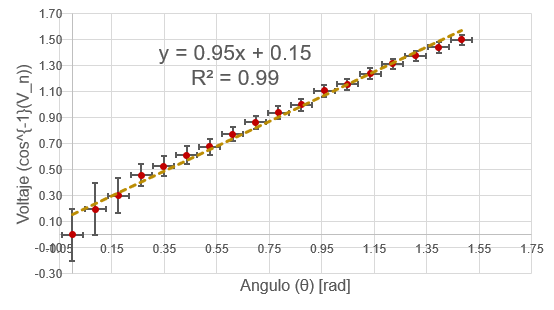
\includegraphics[width=0.3\textwidth]{Lambert1.PNG}}
  \subfloat[\textbf{Gráfica del segundo conjunto de datos normalizados.}Se observa el segundo conjunto de datos obtenidos del experimento con la fuente de LED plano y la ecuación 3.]{
   \label{f:Lambert2}
    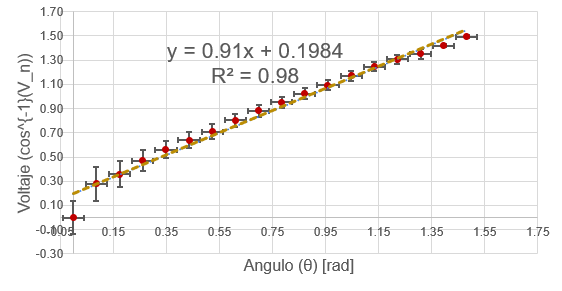
\includegraphics[width=0.3\textwidth]{Lambert2.PNG}}
  \subfloat[\textbf{Gráfica del tercer conjunto de datos normalizados.}Se observa el tercer conjunto de datos obtenidos del experimento con la fuente de LED plano y la ecuación 3.]{
   \label{f:Lambert3}
    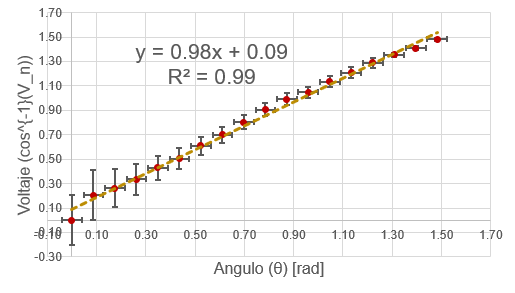
\includegraphics[width=0.3\textwidth]{Lambert3.PNG}}
 \caption{\textbf{Gráficas del Experimento fuente de LED plano.}En ella se muestran las 3 gráficas obtenidas a partir de los datos normalizados (ver apéndice).Se destaca que se ajustaron al modelo lineal de forma favorable. La pendiente de dichas gráficas corresponde al factor de proporcionalidad entre el ángulo y el $\cos^{-1}{V_n}$.}
 \label{f:Lambert}
\end{figure}

De las graficas se obtuvieron las siguientes pendientes:

\begin{equation*}
    m_1 = (0.95 \pm 0.03)
\end{equation*}



\begin{equation*}
    m_2 = (0.91 \pm 0.03)
\end{equation*}



\begin{equation*}
    m_3 = (0.98 \pm 0.02)
\end{equation*}

el promedio de $m_1$, $m_2$, $m_3$ y la incertidumbre sumando por cuadraturas es:

\begin{equation*}
    \hat{m}= 0.95 \pm 0.05
\end{equation*}


\subsection*{\textcolor{carmine}{PARTE II.}}

Utilizando la ecuación 5, $y= \ln{V}$ y $x = \ln{R}$, entonces por la ley de derivación para propagación de incertidumbres:

\begin{equation*}
    \delta y = \sqrt{\left( \frac{\partial y}{\partial V} \delta V \right)^2} = \left|\frac{\partial y}{\partial V}\right| \delta V = \frac{\delta V}{V}
\end{equation*}

\begin{equation*}
    \delta x = \sqrt{\left( \frac{\partial x}{\partial R} \delta R \right)^2} = \left|\frac{\partial x}{\partial R}\right| \delta R = \frac{\delta R}{R}
\end{equation*}
\begin{figure}[H]
 \centering
  \subfloat[\textbf{Gráfica de datos medidos con fuente de luz LED.}\\ Gráfica de los datos medidos en la segunda parte del experimento usando como fuente de luz un LED. En ella se observa la ecuación asociada a la curva obtenida.]{
   \label{f:LED}
    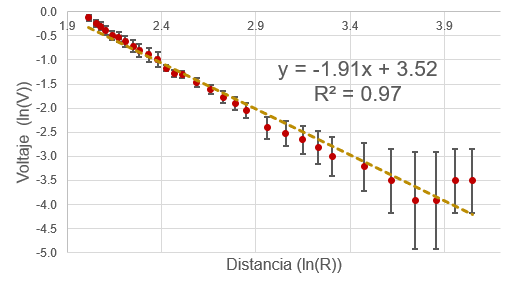
\includegraphics[width=0.5\textwidth]{LED.PNG}}
  \subfloat[\textbf{Gráfica de datos medidos con fuente de luz Láser.}\\Gráfica de los datos medidos en la segunda parte del experimento usando como fuente de luz un láser, en ella se observa la ecuación asociada a la cuerva obtenida.]{
   \label{f:Láser}
    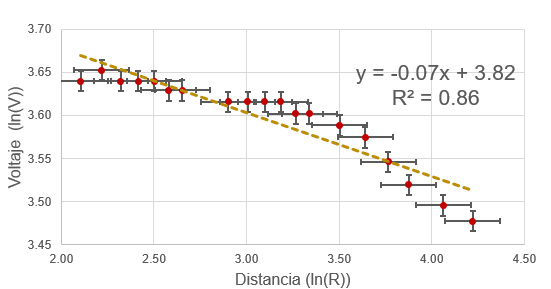
\includegraphics[width=0.5\textwidth]{Laser.PNG}}
    \caption{\textbf{Gráficas de la segunda parte del experimento.} Se muestran las dos gráficas de los datos obtenidos en la segunda parte para el LED 3(a) y el láser 3(b) (ver apéndice), donde la pendiente representa las potencias de las fuentes de luz. Se debe notar que los ejes están en una escala logarítmica.}
 \label{f:Parte 2}
\end{figure}

De la graficas se obtuvo la siguiente pendiente para el LED:

\begin{equation*}
    m = (-1.91 \pm 0.06)
\end{equation*}

Y para el laser:

\begin{equation*}
    m = (-0.07 \pm 0.01)
\end{equation*}
\begin{figure}[H]
    \centering
    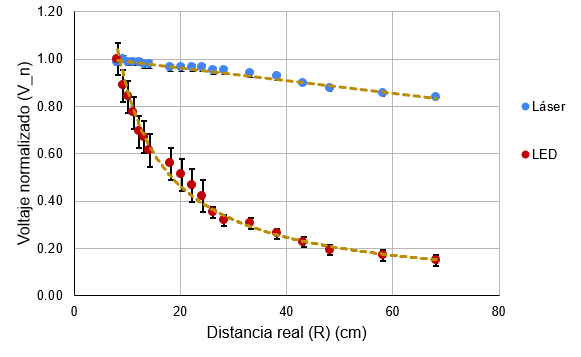
\includegraphics[width=9cm]{LED y LAser.PNG}
    \caption{\textbf{Gráfica de datos normalizados (ver apéndice) para ambas fuentes de luz.} En ella se pueden comparar los comportamientos de ambas fuentes. Se observa la tendencia del Láser a ser constante comparado con la curva de los datos del LED.}
    \label{fig:my_label}
\end{figure}
\newpage
\section*{\textcolor{carmine}{Conclusión.}}
Se obtuvo que una fuente LED plana cumple con la ecuación:

\begin{equation*}
   \cos^{-1}{V_{n}}=(0.95\pm 0.05)\theta  
\end{equation*}

Por lo tanto una fuente LED plana aproxima la Ley coseno de Lambert, como se quería comprobar.
\\\\
También se obtuvo que la fuente LED cumple con:

\begin{equation*}
 % V=\frac{K}{R^{(-1.91\pm0.06)}}
  \ln{V}=(-1.91\pm 0.06)\ln{R}+K_{0}
\end{equation*}


Comparando con la Ley del Inverso al cuadrado:

\begin{equation*}
   \ln{V}= -2\ln{R} + \ln{K}  
\end{equation*}

Se ve que se puede aproximar al LED como una fuente puntual.
\\
\\
%Además nótese que e
El error del resultado obtenido para ley coseno de Lambert es $1$ $(<2)$ veces la incertidumbre absoluta por lo que es satisfactorio, también para la ley del inverso al cuadrado el error es $1.5$ $(<2)$ veces la incertidumbre absoluta por lo que también es satisfactorio.
\\
\\
Para el láser se obtuvo:
$$\ln{V}=(-0.07\pm0.01)\ln{R}+3.82$$
Mientras que para un haz colimado se tiene:
$$ \ln{V}=c $$
Con $c$ constante.
\\
Como para el láser el logaritmo del voltaje varía muy poco, para puntos cercanos, entonces este se puede considerar como una fuente de luz colimada.
\\
La región donde esto se cumple depende de que tan buena se quiera la aproximación. 
\nocite{*}

\bibliography{biblio}
\newpage 
\begin{multicols}{2}
\section*{\textcolor{carmine}{Apéndice}}


\begin{Figura}
    \centering
    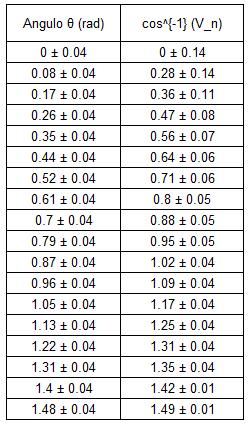
\includegraphics[width=0.4 \textwidth]{tablas/tabla lambert 2.PNG}
    \captionof{table}{Datos normalizados obtenidos con la fuente LED plana graficados en la Figura 4(b).}
    \label{fig}
\end{Figura}

\begin{Figura}
    \centering
    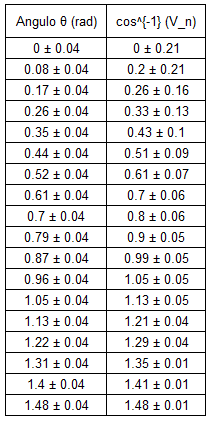
\includegraphics[width=0.4 \textwidth]{tablas/tabla lambert 3.PNG}
    \captionof{table}{Datos normalizados obtenidos con la fuente LED plana graficados en la Figura 4(c).}
    \label{fig}
\end{Figura}

\begin{Figura}
    \centering
    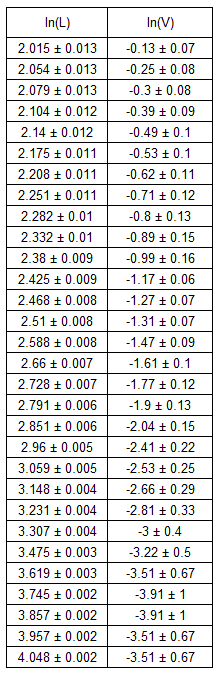
\includegraphics[width=0.4 \textwidth]{tablas/tabla LED.PNG}
    \captionof{table}{Datos obtenidos con la fuente de luz LED graficados en la Figura 5(a).}
    \label{fig}
\end{Figura}

\begin{Figura}
    \centering
    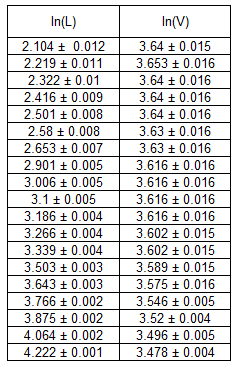
\includegraphics[width=0.4 \textwidth]{tablas/tabla laser.PNG}
    \captionof{table}{Datos obtenidos con la fuente de luz láser graficados en la Figura 5(b).}
    \label{fig}
\end{Figura}

\begin{Figura}
    \centering
    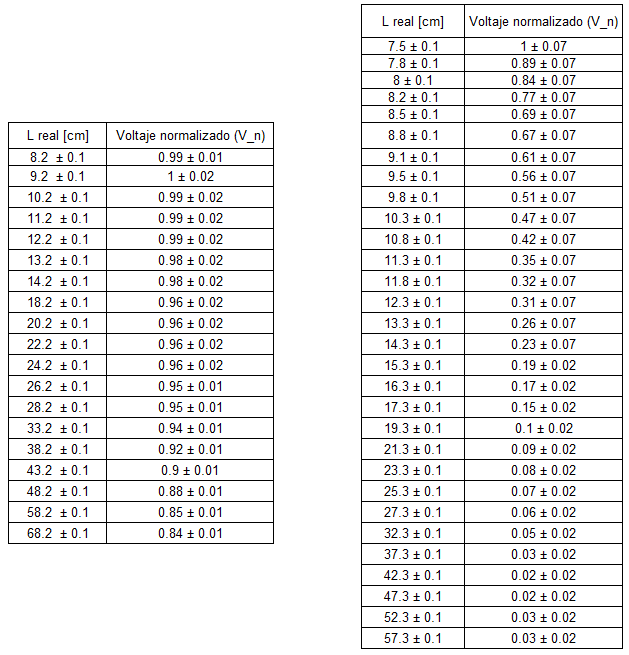
\includegraphics[width=0.5 \textwidth]{tablas/tabla LED laser.PNG}
    \captionof{table}{Datos normalizados de las fuentes de luz LED y láser graficados en la Figura 6}
\end{Figura}


\end{multicols}

\end{document}


